\documentclass[12pt,letterpaper]{article}
\usepackage[utf8]{inputenc}
\usepackage{amsmath, amsfonts, amssymb}
\usepackage{graphicx}
\usepackage[left=2cm,right=2cm,top=2cm,bottom=2cm]{geometry}
\usepackage[margin=20pt,font=small,labelfont=bf,labelsep=period]{caption}
\usepackage{subcaption}


\author{Nicol\'as Guar\'in Zapata}
\title{\textbf{Dispersion relations for spring-mass lattices}}
\begin{document}
\maketitle

%% 
\section{Simple mass-spring lattice}
%Figure
\begin{figure}[h]
\centering
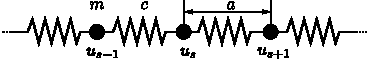
\includegraphics[height=1.5cm]{img/spring-mass.pdf} 
\caption{Simple mass-spring lattice.}
\end{figure}
\subsection{Direct formulation}
The force in the plane $s$ cause by the displacement of the plane $s+p$ is proportional to the difference $u_{s+p}-u_s$ of the displacements. For brevity we will consider only nearest-neighbour interactions, so $p=\pm 1$. The total force on $s$ comes from planes $s=\pm 1$:
\begin{equation}
F_s = c(u_{s+1}-u_s)+ c(u_{s-1}-u_s).
\end{equation}
The constant $c$ is the stiffness between nearest-neighbour planes and will differ for longitudinal and transverse waves.

The equation of motion of the plane $s$ is
\[ m  \ddot{u} = c(u_{s+1} + u_{s-1} -2 u_s), \]
assuming a harmonic time dependence $\exp(-i\omega t)$
\begin{equation}
-m\omega^2 u_s = c(u_{s+1} + u_{s-1} - 2u_s) \enspace .
\label{eq:single-spring-lattice}
\end{equation}
Due to the Bloch-periodicity condition
\[u_{s\pm 1} = u_s e^{\pm i ka}. \]
So (\ref{eq:single-spring-lattice}) is now
\[ -m \omega^2 u_s = c (u_s \exp(ika) + u_s \exp(-ika) - 2u_s) \]
and cancelling $u_s$ from both sides, we have
\[ \omega^2 m = -c[ \exp(ika) + \exp(-ika) - 2 ] \enspace .\]
Using the identity $2\cos ka = \exp(ika) + \exp(-ika)$, we have the dispersion relation
\begin{equation}
\omega^2 = (2c/m) (1-\cos ka) \enspace .
\label{eq:simple-disp-relation}
\end{equation}
The boundary of the first Brillouin zone lies at $k=\pm \pi/a$. We show from (\ref{eq:simple-disp-relation}) that the slope of $\omega$ versus $k$ is zero at the zone boundary
\[ \frac{d\omega^2}{dk} = (2ca/m)\sin ka=0\]
at $k=\pm \pi/a$, $\sin ka = 0$.

By a trigonometric identity (\ref{eq:single-spring-lattice}) may be written as
\begin{equation}
\omega^2 = (4c/m) \sin^2 \frac{1}{2}ka, \qquad \omega = (4c/m)^{1/2}\left\vert \sin \frac{1}{2} ka\right\vert \enspace .
\end{equation}

\begin{figure}[h]
\centering
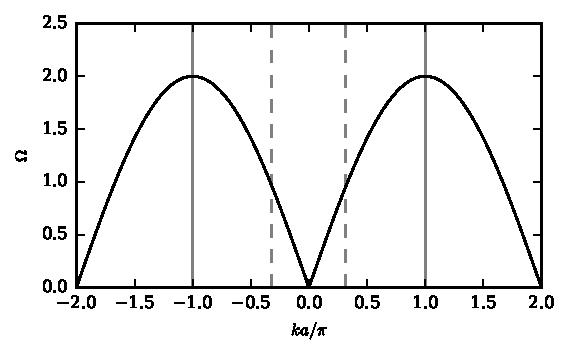
\includegraphics[height=8cm]{img/spring-mass-plot.pdf} 
\caption{Plot of $\omega$ versus $k$. The region of $k<<1/a$ or $\lambda>>a$ corresponds to the continuum approximation; where $\omega$ is directly proportional to k. The First Brillouin Zone is placed between $-\pi/a$ and $\pi/a$.}
\end{figure}

\subsection{Unit cell formulation}
This problem could also be solved taking a single cell and imposing the Bloch conditions after the assemblage process for the matrices. The force balance (in frequency domain) is
\begin{align*}
c(u_2 - u_1) &= -\frac{m}{2} \omega^2 u_1 \enspace ,\\
c(u_1 - u_2) &= -\frac{m}{2} \omega^2 u_2 \enspace ,
\end{align*}
we should take care since the total amount of mass in the cell should be consistent. That's why we choose each particle to have $m/2$. And this system could be expressed as
\begin{equation}
c\left[ \begin{array}{cc}
-1 & 1 \\ 
1 & -1
\end{array}  \right] \left\lbrace \mathbf{u} \right\rbrace =
-\frac{m}{2}\left[ \begin{array}{cc}
1 & 0 \\ 
0 & 1
\end{array}  \right] \left\lbrace \mathbf{u} \right\rbrace \enspace ,
\end{equation}
multiplying the second row by $\exp(-ika)$ and the second column by its complex conjugate $\exp(ika)$ we get
\begin{equation*}
c\left[ \begin{array}{cc}
-1 & e^{ika} \\ 
e^{-ika} & -1
\end{array}  \right] \left\lbrace \mathbf{u} \right\rbrace =
-\frac{m}{2}\left[ \begin{array}{cc}
1 & 0 \\ 
0 & 1
\end{array}  \right] \left\lbrace \mathbf{u} \right\rbrace \enspace ,
\end{equation*}
adding the second row to first one, and then adding the second column to first one yields
\begin{equation*}
c\left[ \begin{array}{cc}
e^{ika}+e^{-ika}-2 & e^{ika}-1 \\ 
e^{-ika}-1 & -1
\end{array}  \right] \left\lbrace \mathbf{u} \right\rbrace =
-\frac{m}{2}\left[ \begin{array}{cc}
2 & 1 \\ 
1 & 1
\end{array}  \right] \left\lbrace \mathbf{u} \right\rbrace \enspace .
\end{equation*}
Now, were interested just in the reduced system, we delete the second row and column and get
\begin{equation}
\frac{c}{m}\left[ e^{ika}+e^{-ika}-2 \right] = \omega^2 \enspace ,
\end{equation}
and this could be rewritten as
\begin{equation}
\omega = (4c/m)^{1/2}\left\vert \sin \frac{1}{2} ka\right\vert \enspace ,
\end{equation}
which is the same result obtained before.

%% 
\section{Diatomic crystal}
\begin{figure}[h]
\centering
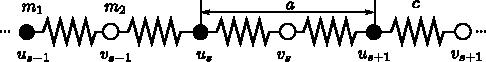
\includegraphics[height=1.5cm]{img/diatomic-crystal.pdf} 
\caption{Lattice made with spring and two species of masses.}
\end{figure}
We write the equations of motion under the assumption that each plane interacts only with its nearest-neighbour planes and that the force constants are identical between all pairs of nearest-neighbour planes.
\begin{subequations}
\begin{align}
m_1\frac{d^2 u_s}{dt^2} = c(v_s+v_{s-1}-2u_s); \\
m_2\frac{d^2 v_s}{dt^2} = c(u_{s+1}+u_{s}-2v_s).
\end{align}
\label{eq:diatomic-eq}
\end{subequations}
We look for a solution in the form of a traveling wave, now with different amplitudes $u$, $v$ on alternate phases:
\begin{subequations}
\begin{align}
u_s = u\exp(ika)\exp(-i\omega t); \\
v_s = v\exp(ika)\exp(-i\omega t).
\end{align}
\label{eq:diatomic-sol}
\end{subequations}
Replacing (\ref{eq:diatomic-sol}) in (\ref{eq:diatomic-eq}) we have
\begin{align*}
-\omega^2 m_1 u = cv[1+\exp(-ika)] - 2cu; \\
-\omega^2 m_2 v = cu[1+\exp(ika)] - 2cv.
\end{align*}
It has no trivial solution only if the determinant vanishes, i.e.
\[\left\vert \begin{array}{cc}
2c - m_1 \omega^2 & -c[1+\exp(-ika)] \\ 
-c[1+\exp(ika)] & 2c - m_2 \omega^2
\end{array}  \right\vert = 0,\]
or
\begin{equation}
m_1 m_2 \omega^4 - 2c(m_1 + m_2)\omega^2 + 2c^2(1-\cos ka)=0 \enspace .
\end{equation}
Solving this biquadratic equation and doing some algebraic manipulations, we get
\begin{equation}
\omega^2 = \frac{c}{m_1 m_2} \left[ m_1+m_2 \pm \sqrt{(m_1+m_2)^2-2m_1 m_2(1-\cos ka)}\right] \enspace .
\end{equation}
\begin{figure}[h]
\centering
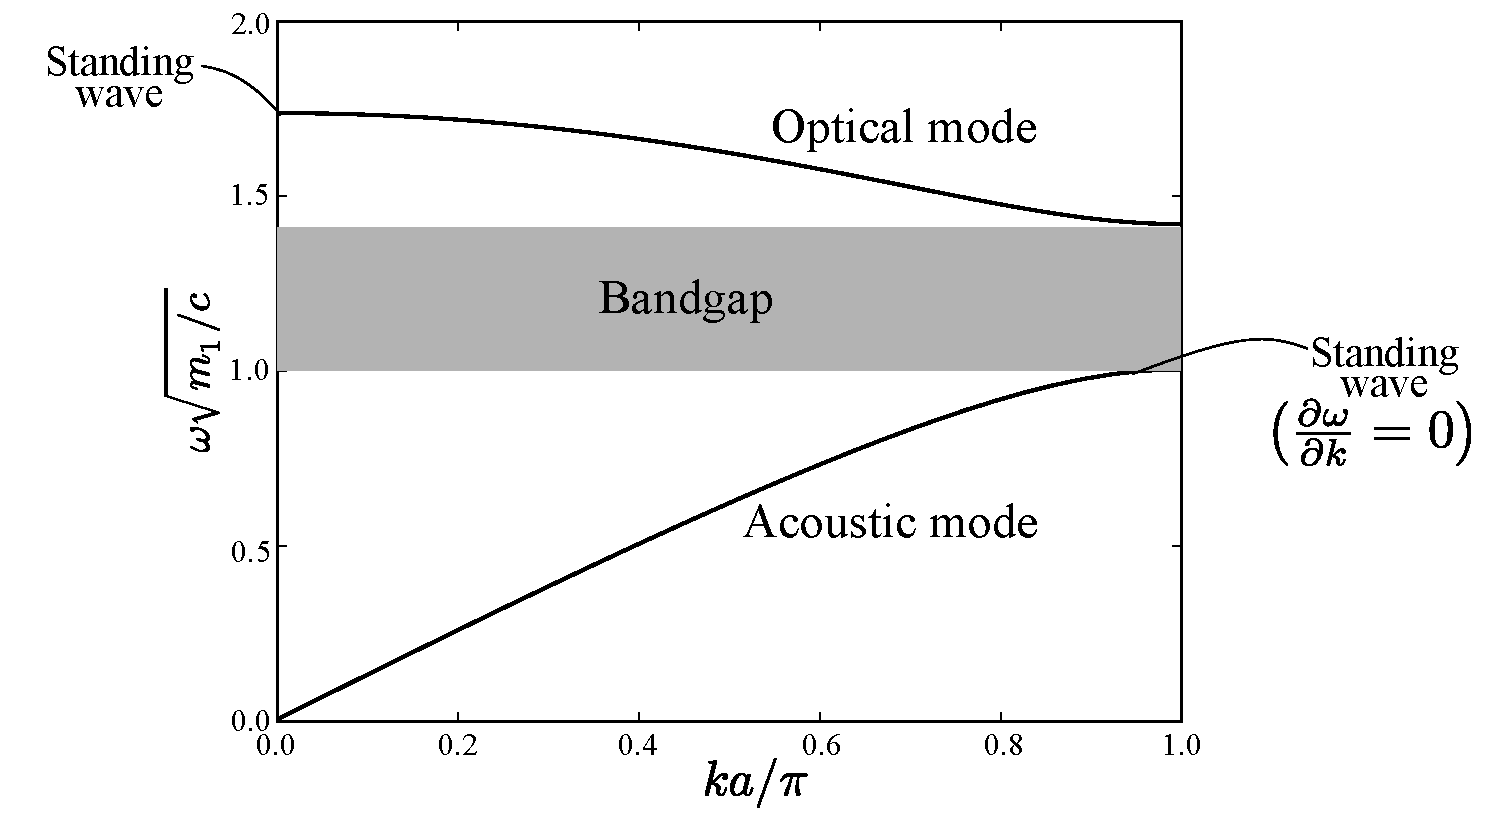
\includegraphics[height=8cm]{img/diatomic-plot.pdf} 
\caption{Optical and acoustical branches of the dispersion relation for a diatomic linear lattice. The values are computed for a ratio $m_2/m_1 = 2$.}
\end{figure}
Let's examine the limiting cases $ka<<1$ and $ka=\pm \pi$ at the boundary zone. For small $ka$ we have $\cos ka \approx 1 - \frac{1}{2}k^2a^2 + \cdots$, and the two roots are
\begin{align}
\omega^2 &\approx 2c\left(\frac{1}{m_1} + \frac{1}{m_2}\right)\quad \mbox{(optical branch)}\\
\omega^2 &\approx \frac{\frac{1}{2}c}{m_1+m_2}k^2a^2\quad \mbox{(acoustical branch)} \enspace  .
\end{align}
At $k_{max}=\pm\pi/a$ the roots are
\[\omega^2 = 2c/m_1,\quad \omega^2 = 2c/m_2 \enspace .\]

\section{Three masses lattice}
The equations are
\begin{subequations}
\begin{align}
m_1\frac{d^2 u_s}{dt^2} = c(v_s+w_{s-1}-2u_s); \\
m_2\frac{d^2 v_s}{dt^2} = c(w_{s}+u_{s}-2v_s);\\
m_3\frac{d^2 w_s}{dt^2} =c(u_{s+1}+v_{s}-2w_s).
\end{align}
\label{eq:three-masses}
\end{subequations}
After assume an harmonic solution and apply Bloch conditions the following system is found
 \begin{equation}
\left[ \begin{array}{ccc}
-2 & 1 & \exp(-ika) \\ 
1 & -2 & 1 \\ 
\exp(ika) & 1 & -2
\end{array}  \right] \left\lbrace \begin{array}{c}
u \\ 
v \\ 
w
\end{array}  \right\rbrace = -\frac{\omega^2}{\omega_0^2}\left[ \begin{array}{ccc}
1 & 0 & 0 \\ 
0 & \mu_1 & 0 \\ 
0 & 0 & \mu_2
\end{array} \right] \left\lbrace \begin{array}{c}
u \\ 
v \\ 
w
\end{array} \right\rbrace \enspace , 
 \end{equation}
where $\omega_0^2=c/m_1$, $\mu_1 = m_2/m_1$ and $\mu_2=m_3/m_1$. The characteristic polynomial for this system is
\begin{equation}
\mu_1 \mu_2 x^3 - 2[\mu_1\mu_2 -\mu_1 -\mu_2]x^2 + 3[\mu_1+\mu_2+1]x+2[\cos ka -1] = 0 \enspace .
\end{equation}
Figure \ref{fig:three-masses} presents some dispersion curves for different mass ratios.
\begin{figure}[h]
        \centering
        \begin{subfigure}[b]{0.49\textwidth}
                \includegraphics[width=\textwidth]{img/{spring_masses-3-m1=0.5-m2=3}.pdf}
                \caption{$\mu_1=1/2$, $\mu_2=3$.}
        \end{subfigure}\,
%
        \begin{subfigure}[b]{0.49\textwidth}
                \includegraphics[width=\textwidth]{img/{spring_masses-3-m1=0.5-m2=10}.pdf}
                \caption{$\mu_1=1/2$, $\mu_2=10$.}
        \end{subfigure}\\
%
        \begin{subfigure}[b]{0.49\textwidth}
                \includegraphics[width=\textwidth]{img/{spring_masses-3-m1=2-m2=3}.pdf}
                \caption{$\mu_1=2$, $\mu_2=3$.}
        \end{subfigure}\,
%
        \begin{subfigure}[b]{0.49\textwidth}
                \includegraphics[width=\textwidth]{img/{spring_masses-3-m1=2-m2=10}.pdf}
                \caption{$\mu_1=2$, $\mu_2=10$.}
        \end{subfigure}
        \caption{Dispersion curves for different values of mass ratios $\mu_1, \mu_2$.}\label{fig:three-masses}
\end{figure}

\section{2D square lattice}
For the simple cases shown before is easy to formulate the complete balance of forces taking into account the first neighbours. In general is easier to take the unit cell for the lattice and find the resulting system through row and column operations, just as exemplified before. 
\begin{figure}[h]
\centering
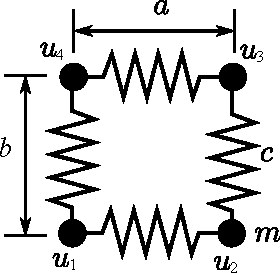
\includegraphics[height=5cm]{img/spring-square.pdf} 
\caption{Unit cell for a two dimensional square lattice with a unique species.}
\end{figure}
The system of equation in frequency domain is
\begin{equation}
c\left[ \begin{array}{cccccccc}
-1 & 0 & 1 & 0 & 0 & 0 & 0 & 0 \\ 
0 & -1 & 0 & 0 & 0 & 0 & 0 & 1 \\ 
1 & 0 & -1 & 0 & 0 & 0 & 0 & 0 \\ 
0 & 0 & 0 & -1 & 0 & 1 & 0 & 0 \\ 
0 & 0 & 0 & 0 & -1 & 0 & 1 & 0 \\ 
0 & 0 & 0 & 1 & 0 & -1 & 0 & 0 \\ 
0 & 0 & 0 & 0 & 1 & 0 & -1 & 0 \\ 
0 & 1 & 0 & 0 & 0 & 0 & 0 & -1
\end{array} \right] \left\lbrace \begin{array}{c}
u_1 \\ 
v_1 \\ 
u_2 \\ 
v_2 \\ 
u_3 \\ 
v_3 \\ 
u_4 \\ 
v_4
\end{array}  \right\rbrace= -\frac{\omega}{4}m \mathbb{I}_8
\left\lbrace \begin{array}{c}
u_1 \\ 
v_1 \\ 
u_2 \\ 
v_2 \\ 
u_3 \\ 
v_3 \\ 
u_4 \\ 
v_4
\end{array}  \right\rbrace \enspace ,
\end{equation}
and after applying the row operations for the Bloch-conditions imposition, we get
\begin{equation}
\frac{4c}{m}\left[ \begin{array}{cc}
1 - \cos(k_x a) & 0 \\ 
0 & 1-\cos(k_y b)
\end{array}  \right] \left\lbrace \begin{array}{c}
u_1 \\ 
v_1 
\end{array}  \right\rbrace = \omega^2 \left\lbrace \begin{array}{c}
u_1 \\ 
v_1 
\end{array}  \right\rbrace .
\end{equation}
Or, equivalently
\begin{equation}
\omega_x^2 = \frac{8c}{m}\left( \sin \frac{1}{2}k_x a\right)^2,\qquad \omega_y^2 = \frac{8c}{m}\left( \sin \frac{1}{2}k_y b \right)^2 \enspace .
\end{equation}
\begin{figure}[h]
\centering
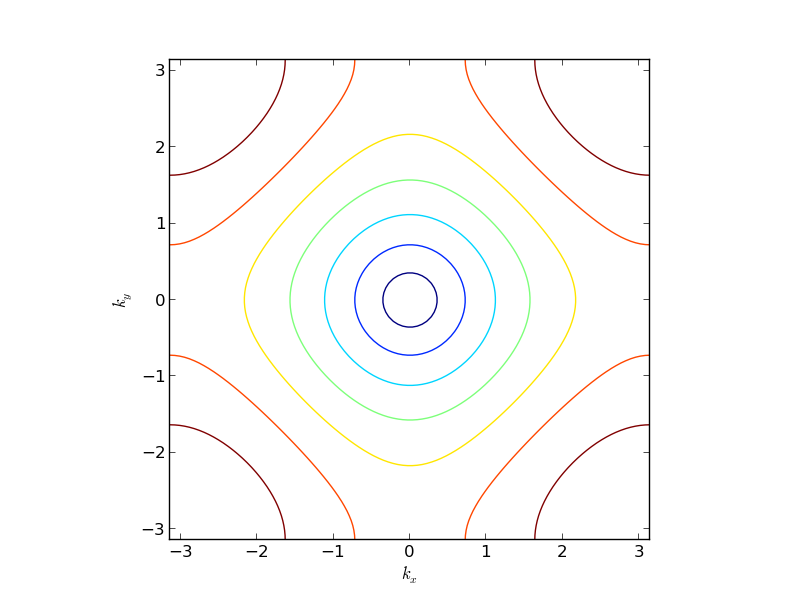
\includegraphics[height=8cm]{img/square-mass_lattice-contours.png} 
\caption{Isofrequency contours for the first mode.}
\end{figure}

\section{2D square lattice with diagonal springs}
\begin{figure}[h]
\centering
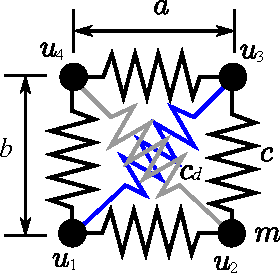
\includegraphics[height=5cm]{img/spring-square-diag.pdf} 
\caption{Unit cell for a two dimensional square lattice with a unique species and diagonal springs.}
\end{figure}

The system of equation in frequency domain is
\begin{equation}
\mathbb{K}
\left\lbrace \begin{array}{c}
u_1 \\ 
v_1 \\ 
u_2 \\ 
v_2 \\ 
u_3 \\ 
v_3 \\ 
u_4 \\ 
v_4
\end{array}  \right\rbrace= -\frac{\omega^2}{4}m \mathbb{I}_8
\left\lbrace \begin{array}{c}
u_1 \\ 
v_1 \\ 
u_2 \\ 
v_2 \\ 
u_3 \\ 
v_3 \\ 
u_4 \\ 
v_4
\end{array} \right\rbrace
\end{equation}
with
\[\mathbb{K} = \begin{bmatrix}
-c_{d}-c_{1} & 0 & c_{1} & 0 & c_{d} & 0 & 0 & 0\cr
0 & -c_{d}-c_{2} & 0 & 0 & 0 & c_{d} & 0 & c_{2}\cr
c_{1} & 0 & -c_{d}-c_{1} & 0 & 0 & 0 & c_{d} & 0\cr
0 & 0 & 0 & -c_{d}-c_{2} & 0 & c_{2} & 0 & c_{d}\cr
c_{d} & 0 & 0 & 0 & -c_{d}-c_{1} & 0 & c_{1} & 0\cr
0 & c_{d} & 0 & c_{2} & 0 & -c_{d}-c_{2} & 0 & 0\cr
0 & 0 & c_{d} & 0 & c_{1} & 0 & -c_{d}-c_{1} & 0\cr
0 & c_{2} & 0 & c_{d} & 0 & 0 & 0 & -c_{d}-c_{2}\end{bmatrix} \]

And the solutions are
\begin{align*}
\omega_1^2 &= \frac{4c_1}{m}\left[1 - \cos k_x a \right] + \frac{4 c_d}{m}\left[1 - \cos k_x a \cos k_y b \right]\\
\omega_2^2 &= \frac{4c_2}{m}\left[1 - \cos k_y a \right] + \frac{4 c_d}{m}\left[1 - \cos k_x a \cos k_y b \right] \enspace .
\end{align*}
equivalently (after some manipulations)
\begin{align}
\omega_1^2 &= \frac{8c_1}{m} \sin^2 \left(\frac{1}{2}k_x a\right)  + \frac{4c_d}{m} \left[\sin^2 \frac{1}{2}\left(k_x a + k_y b\right) + \sin^2 \frac{1}{2}\left(k_x a - k_y b\right)\right] \\
\omega_2^2 &= \frac{8c_2}{m} \sin^2 \left(\frac{1}{2}k_y b\right)  + \frac{4c_d}{m} \left[\sin^2 \frac{1}{2}\left(k_x a + k_y b\right) + \sin^2 \frac{1}{2}\left(k_x a - k_y b\right)\right]  
\end{align}
We recover the square lattice (without diagonals) making $c_d=0$.


\section{2D square lattice with body mass and diagonal springs}
\begin{figure}[h]
\centering
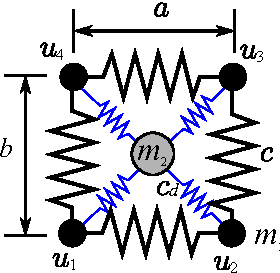
\includegraphics[height=5cm]{img/spring-square-bcc.pdf} 
\caption{Unit cell for a two dimensional square lattice with a unique species in the corners and another one in the center that is linked by diagonal springs.}
\end{figure}
\begin{equation}
\mathbb{K}
\left\lbrace \begin{array}{c}
u_1 \\ 
v_1 \\ 
u_2 \\ 
v_2 \\ 
u_3 \\ 
v_3 \\ 
u_4 \\ 
v_4 \\
u_5 \\
v_5
\end{array}  \right\rbrace= -\omega^2 \mathbb{M}
\left\lbrace \begin{array}{c}
u_1 \\ 
v_1 \\ 
u_2 \\ 
v_2 \\ 
u_3 \\ 
v_3 \\ 
u_4 \\ 
v_4
u_5 \\
v_5
\end{array} \right\rbrace
\end{equation}
with
\[\mathbb{K} =\begin{bmatrix}
-{c}_{s}-{c}_{d} & 0 & {c}_{s} & 0 & 0 & 0 & 0 & 0 & {c}_{d} & 0\cr
 0 & -{c}_{s}-{c}_{d} & 0 & 0 & 0 & 0 & 0 & {c}_{s} & 0 & {c}_{d}\cr
 {c}_{s} & 0 & -{c}_{s}-{c}_{d} & 0 & 0 & 0 & 0 & 0 & {c}_{d} & 0\cr
 0 & 0 & 0 & -{c}_{s}-{c}_{d} & 0 & {c}_{s} & 0 & 0 & 0 & {c}_{d}\cr
 0 & 0 & 0 & 0 & -{c}_{s}-{c}_{d} & 0 & {c}_{s} & 0 & {c}_{d} & 0\cr
 0 & 0 & 0 & {c}_{s} & 0 & -{c}_{s}-{c}_{d} & 0 & 0 & 0 & {c}_{d}\cr
 0 & 0 & 0 & 0 & {c}_{s} & 0 & -{c}_{s}-{c}_{d} & 0 & {c}_{d} & 0\cr
 0 & {c}_{s} & 0 & 0 & 0 & 0 & 0 & -{c}_{s}-{c}_{d} & 0 & {c}_{d}\cr
 {c}_{d} & 0 & {c}_{d} & 0 & {c}_{d} & 0 & {c}_{d} & 0 & -4\,{c}_{d} & 0\cr
 0 & {c}_{d} & 0 & {c}_{d} & 0 & {c}_{d} & 0 & {c}_{d} & 0 & -4\,{c}_{d}\end{bmatrix},\]
and
\[\mathbb{M} = \begin{bmatrix}
\frac{m_1}{4}\mathbb{I}_6 & 0 \\ 
0 & m_2\mathbb{I}_2
\end{bmatrix} \enspace . \]

After applying the Bloch theorem we obtain (showing just the lower diagonal due to the Hermiticity)
\[\mathbb{K}_R = \begin{bmatrix}
-4\left[c_d - c_s(\cos(k_y a) - 1)\right]  & \bullet & \bullet & \bullet\\
 0 & -4\left[c_d - c_s(\cos(k_y b) - 1)\right]  & \bullet & \bullet\\
 c_d\left( e^{i\, k_x a}+1\right) \left( e^{i\, k_y b}+1\right)  & 0 & -4c_d & \bullet\\
 0 & c_d\left( e^{i\, k_x a}+1\right) \left( e^{i\, k_y b}+1\right)  & 0 & -4c_d
\end{bmatrix}\]
and
\[\mathbb{M}_R =\begin{bmatrix}
m_1\mathbb{I}_2 & 0 \\ 
0 & m_2\mathbb{I}_2
\end{bmatrix} \enspace .\]

The eigenvalues for this problem are lengthy, but a second order expansion around $(k_x,k_y)=(0,0)$ (linear in the case o its square root) is shown
\begin{align*}
\omega_1^2 =& \frac{2c_s (k_x a)^2 + c_d\left((k_x a)^2 + (k_y b)^2\right)}{m_1 + m_2}\\
\omega_2^2 =& \frac{2c_s (k_y b)^2 + c_d\left((k_x a)^2 + (k_y b)^2\right)}{m_1 + m_2}\\
\omega_3^2 =& \frac{2c_s (k_x a)^2 + 2c_d\left[2m_1^2 + 2m_2^2 + \left(4 - (k_x a)^2 +(k_y b)^2\right)m_1 m_2\right] } {m_1 m_2 (m_2 + m_1)}\\
\omega_4^2 =& \frac{2c_s (k_y b)^2 + 2c_d\left[2m_1^2 + 2m_2^2 + \left(4 - (k_x a)^2 +(k_y b)^2\right)m_1 m_2\right] } {m_1 m_2 (m_2 + m_1)} \enspace .
\end{align*}
Assuming $a=b$, we can group the modes as degenerate ones and consider the most general propagation in the plane (due to the orthogonality)
\[\omega_{\text{low}}^2 = \frac{2 (c_s + c_d) (k_x^2 + k_y^2)a^2}{m_1 + m_2} \equiv \frac{2 (c_s + c_d) \mathbf{k}^2 a^2}{m_1 + m_2} \enspace ,\]
the same argument holds for the other two, giving
\[\omega_{\text{high}}^2 = \frac{2c_s \mathbf{k}^2a^2 + 2c_d\left[4m_1^2 + 4m_2^2 + \left(8 - \mathbf{k}^2 a^2\right)m_1 m_2\right] } {m_1 m_2 (m_2 + m_1)} \enspace .\]


\end{document}

